%4.	Given the large number of related outcomes (e.g., Figure 2), the authors may want to consider adjustments for multiple hypothesis testing.


We thank the reviewer for this suggestion.

We acknowledge that testing multiple outcomes simultaneously raises concerns about false discoveries. We note, however, that all six outcomes in our main analysis---including the four now presented in Figure 2 and the arrests and trust-in-police outcomes moved to the mechanisms section in the revised manuscript---are statistically significant at the 1\% significance level. Under the null hypothesis of no effects, one would expect at most 1\% of tested coefficients to be false positives by chance at the same level. The observed pattern of results is therefore difficult to reconcile with false discoveries driven by multiple testing. Nonetheless, to address this concern formally, we apply a multiple hypothesis testing correction to the p-values. While procedures such as \citet{romano2005} would be the natural choice, their implementation is not computationally straightforward with the \citet{Callaway} estimator. We therefore apply the Bonferroni correction, which can be applied directly to any set of estimated p-values regardless of the underlying estimator. The adjusted p-values, reported in Table \ref{tab:bonferroni}, confirm that the main results remain statistically significant after correction for every outcome considered. 

In the revised manuscript, we have added the following footnote in Section 4.1: 


\begin{adjustwidth}{2em}{0em}
Table \ref{tab:bonferroni} in Online Appendix \ref{sec:appendixC} applies the Bonferroni correction across the main outcome estimates and confirms that these results are not a product of multiple hypothesis testing.
\end{adjustwidth}

We also add the following subsection, ``Multiple Hypothesis Testing,'' to Online Appendix C reporting this exercise in detail:

\begin{adjustwidth}{2em}{0em}
Testing multiple outcomes simultaneously raises concerns about false discoveries. In our analyses, all six outcomes in our main analyses are statistically significant at the 1\% significance level. Under the null hypothesis of no effects, one would expect at most 1\% of tested coefficients to be false positives by chance at the same level. The observed pattern of results is therefore difficult to reconcile with false discoveries driven by multiple testing. Nonetheless, to address this concern formally, we apply a multiple hypothesis testing correction to the p-values. While procedures such as \citet{romano2005} would be a natural choice, their implementation is not computationally straightforward with the \citet{Callaway} estimator. We therefore apply the Bonferroni correction, which can be applied directly to any set of estimated p-values regardless of the underlying estimator. The adjusted p-values, reported in Table \ref{tab:bonferroni}, confirm that the main results remain statistically significant at conventional confidence levels after correction for every outcome considered.
\end{adjustwidth}

\clearpage
\noindent\textbf{Other figure and table referenced above:}
\vspace{0.5em}

{\setcounter{figure}{1}\renewcommand{\thefigure}{\arabic{figure}}
%--- Implementation
\begin{figure}[h!]
    \centering
    \caption{Effects of \emph{Plan Cuadrante} on Crime Outcomes and Security Perceptions}
    \label{fig:figure02}
    \begin{subfigure}{0.495\textwidth}
        \centering
        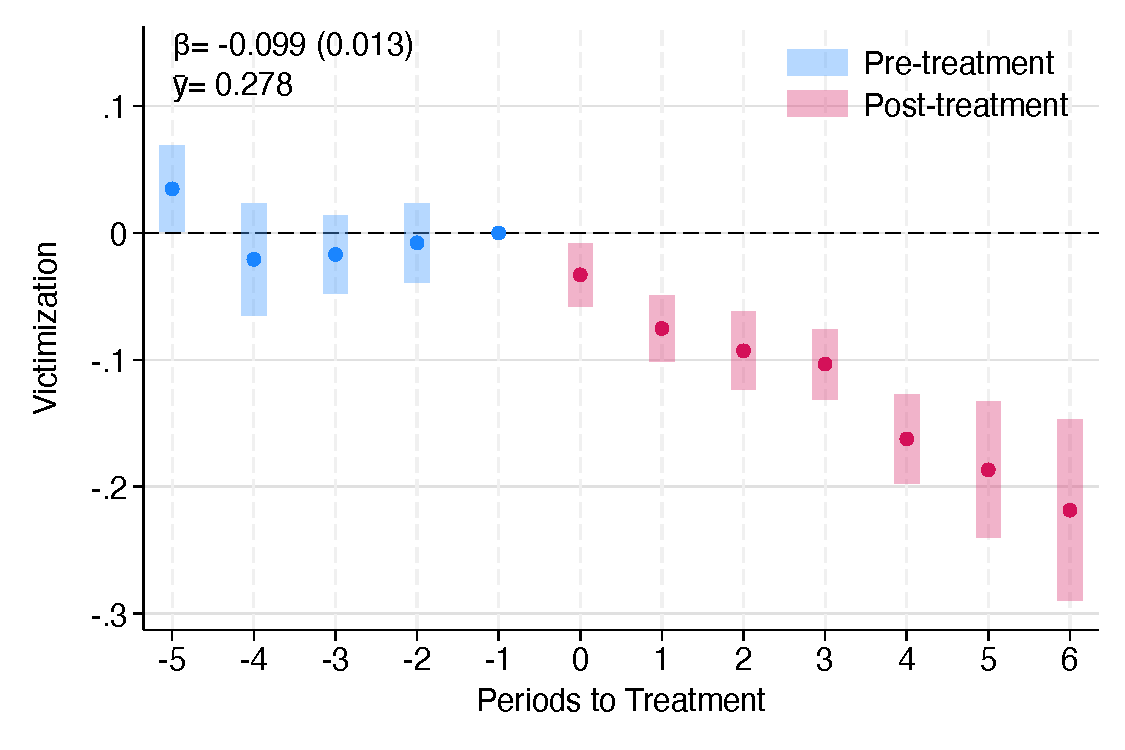
\includegraphics[width=\textwidth]{../manuscript/Graphs/results_victimization.pdf}
        \caption{Victimization in last 12 months}
    \end{subfigure}%
    ~
    \begin{subfigure}{0.495\textwidth}
    \centering
    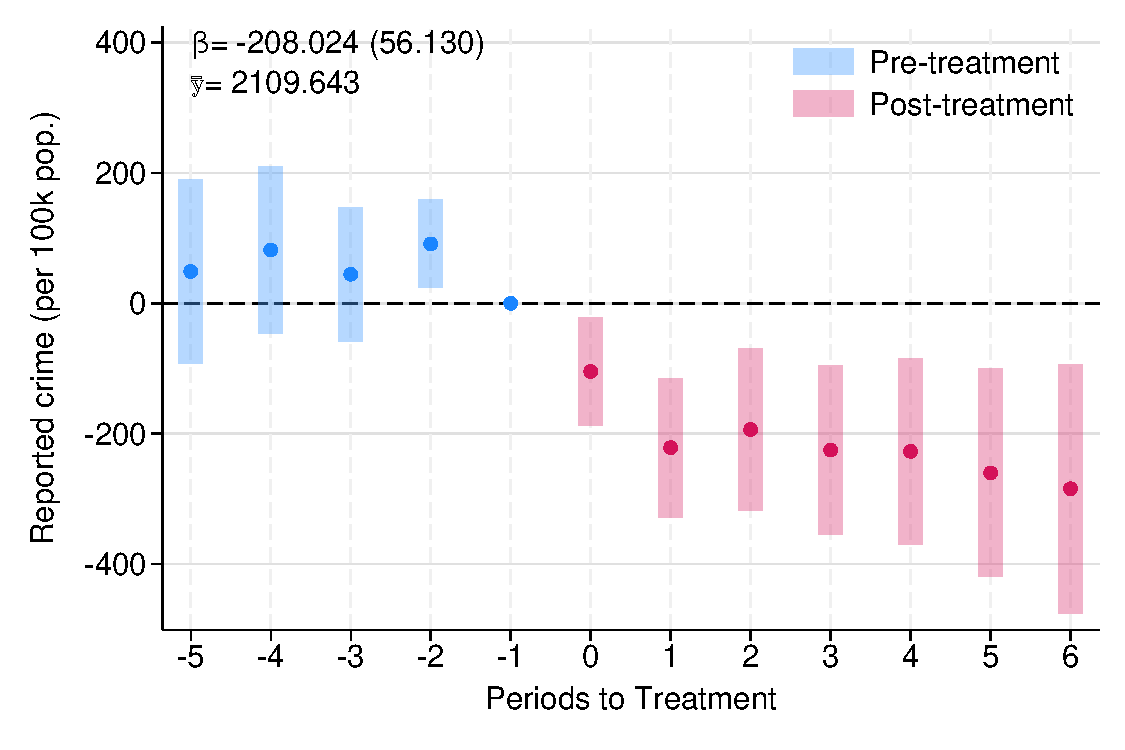
\includegraphics[width=\textwidth]{../manuscript/Graphs/totalreportedcrime_allcomunas.pdf}
        \caption{Reported crime per 100k inhabitants}
    \end{subfigure}
        \begin{subfigure}{0.495\textwidth}
        \centering
        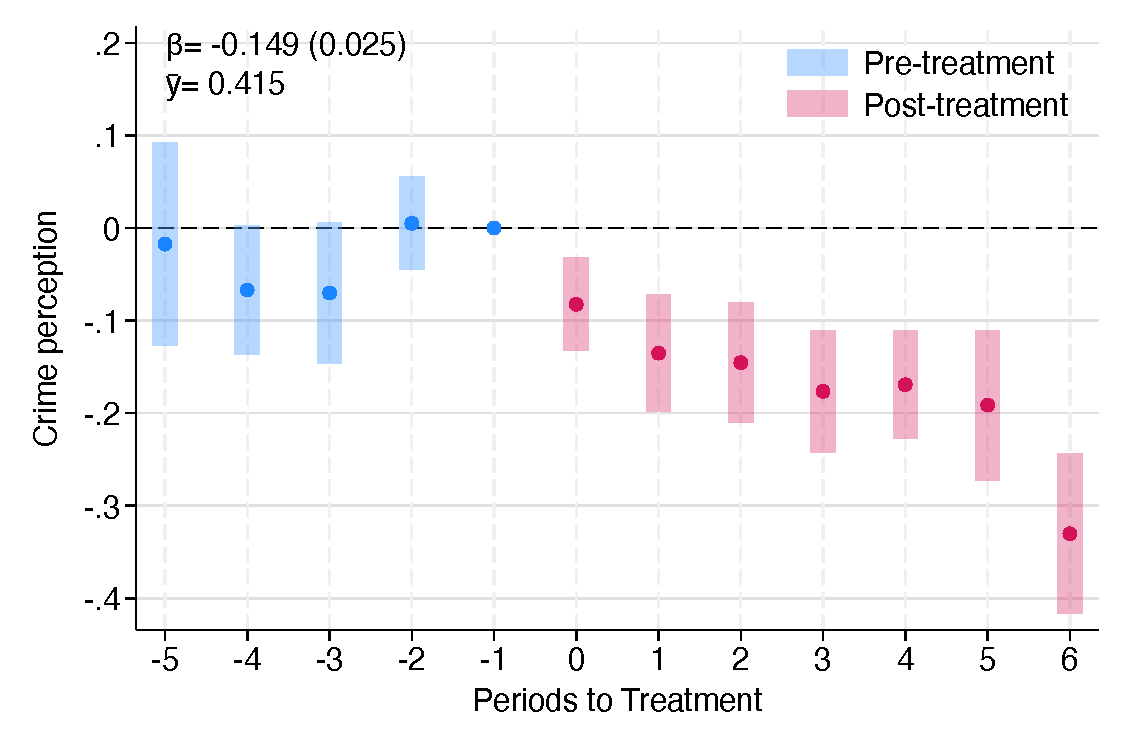
\includegraphics[width=\textwidth]{../manuscript/Graphs/results_perception.pdf}
        \caption{Households reporting an increase in crime}
    \end{subfigure}%
    ~
    \begin{subfigure}{0.495\textwidth}
    \centering
    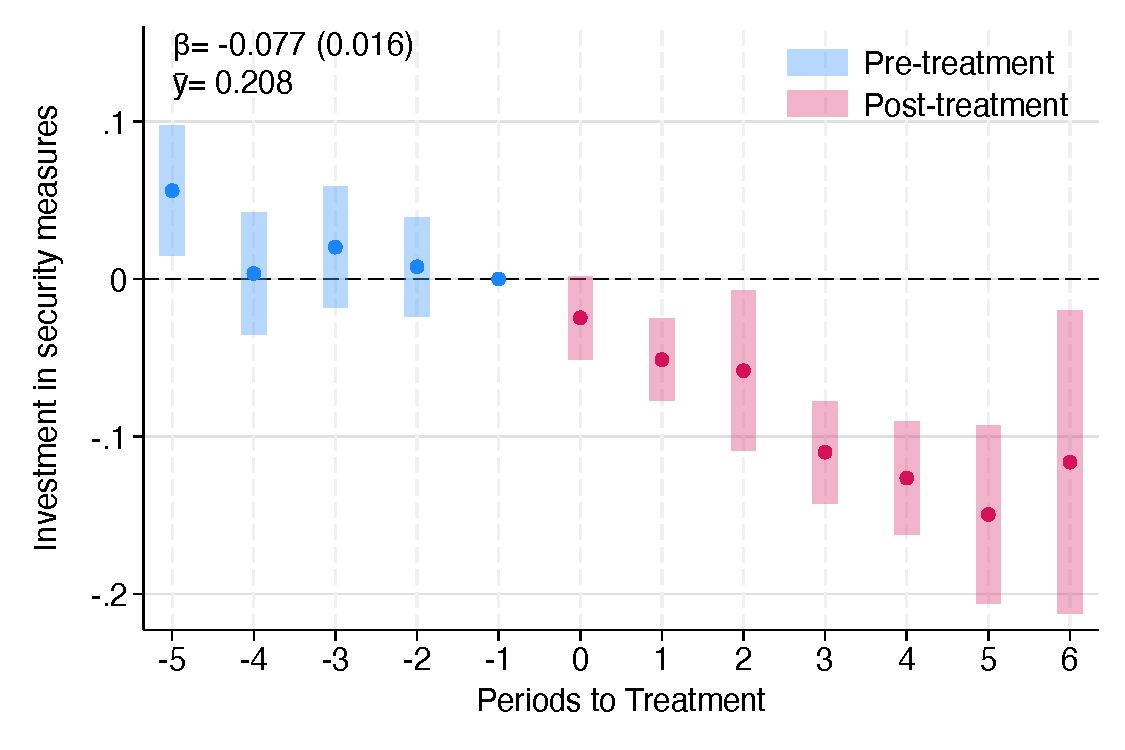
\includegraphics[width=\textwidth]{../manuscript/Graphs/results_hhprotectionmeasures.pdf}
        \caption{Households adopting security measures}
    \end{subfigure}
    \\[12pt]
    \begin{minipage}{0.99\textwidth}
    \footnotesize
    Notes: This figure shows the dynamic effects of the \emph{Plan Cuadrante} on different measures of police effectiveness. The estimation is conducted using the procedure developed in \citet{Callaway} for difference-in-differences with staggered treatment adoption. The dots in the figure represent the estimated coefficients and the bars behind them 95\% confidence intervals. Standard errors are clustered at the municipality level using the wild bootstrapping procedure. The pooled effect and the mean outcome before the introduction of the treatment is also presented in each panel. Panel (a) reports the effect of \emph{Plan Cuadrante} on the probability of household victimization in the last 12 months using the ENUSC survey. Panel (b) reports the effect on the number of crimes reported to the police in the municipality per 100,000 inhabitants using administrative data. Panel (c) reports the effect on the probability of perceiving an increase in crime using the ENUSC survey. Panel (d) reports the effect on the probability of adopting security measures in the last twelve months using the ENUSC survey. Panel (a) includes 93,041 observations; panel (b), 4,231; panel (c), 89,578; and panel (d), 93,041 observations.
    \end{minipage}
\end{figure}
}

\clearpage

{\renewcommand{\thetable}{C.2}
\begin{table}[H]
\centering
\caption{Multiple Hypothesis Testing: Bonferroni Correction}
\label{tab:bonferroni}
\begin{tabular}{lcccc}
\toprule
Outcome & \multicolumn{2}{c}{} & \multicolumn{2}{c}{Bonferroni} \\
 & \multicolumn{2}{c}{Original} & \multicolumn{2}{c}{adjusted} \\
\cmidrule(lr){2-3} \cmidrule(lr){4-5}
 & p-value & & p-value & \\
\midrule
Victimization & 0.00000 & *** & 0.00000 & *** \\
Reported crime (per 100k pop.) & 0.00021 & *** & 0.00126 & *** \\
Crime perception & 0.00000 & *** & 0.00000 & *** \\
Investment in security measures & 0.00000 & *** & 0.00000 & *** \\
Trust in the police & 0.00000 & *** & 0.00000 & *** \\
Arrests (per 100k pop.) & 0.00316 & *** & 0.01896 & ** \\
\midrule
\multicolumn{5}{l}{\footnotesize Notes: Bonferroni correction multiplies each p-value by the number of} \\
\multicolumn{5}{l}{\footnotesize outcomes tested ($n=6$). Significance levels: *** $p<0.01$, ** $p<0.05$, * $p<0.1$.}
\end{tabular}
\end{table}}

\clearpage


